%% LaTeX2e class for student theses
%% sections/content.tex
%% 
%% Karlsruhe Institute of Technology
%% Institute for Program Structures and Data Organization
%% Chair for Software Design and Quality (SDQ)
%%
%% Dr.-Ing. Erik Burger
%% burger@kit.edu
%%
%% Version 1.1, 2014-11-21

\chapter{Grundlagen}
\label{ch:grundlagen}
Die Bachelorarbeit setzt konzeptionell im Wesentlichen auf drei existierenden Grundlagen auf. Dabei soll zunächst eine Erweiterung der Architekturbeschreibungssprache Palladio \cite{Becker2010} erstellt werden, die das Paradigma der komponentenbasierten Entwicklung \cite{Koziolek2006} und ihr Rollenverständnis zugrunde legt. Der Gesamtansatz lässt sich in den Bereich der modellgetriebenen Entwicklung \cite{Stahl2007} einordnen. In den folgenden Abschnitten werden diese Konzepte kurz erläutert.

\section{Modellgetriebene Software-Entwicklung}
\label{sec:modellgetriebeneSE}
In der modellgetriebenen Software-Entwicklung \cite{Stahl2007} werden Teile des Software-Systems innerhalb von Modellen unter Nutzung von Abstraktionen beschrieben. Modelle sind Entwicklungsartefakte und Systembestandteile oder erlauben das automatische Ableiten von Systemartefakten. Das Ziel der modellgetriebenen Softwareentwicklung ist, die Verbesserung der Softwarequalität und der Wiederverwendbarkeit. Außerdem soll eine Erhöhung der Entwicklungseffizienz, zum Beispiel durch Quellcodeerzeugung, aus den Modellen erreicht werden. 

\subsection{Modell}
\label{sec:Modell}
Nach Herbert Stachowiak \cite{Stachowiak1973} zeichnet sich ein Modell durch die folgenden drei Merkmale aus.
\begin{itemize}
\item \textbf{Abbildung} - Bei einem Modell handelt es sich um eine Abbildung oder Repräsentation von einem künstlichen oder natürlichen Original. Das Original kann selbst wieder ein Modell sein. 
\item \textbf{Verkürzung} - Es werden nicht alle Attribute des Originals erfasst, sondern nur diejenigen, die relevant sind.
\item \textbf{Pragmatismus} - Modelle erfüllen ihre Ersatzfunktion für bestimmte Subjekte, innerhalb einer bestimmten Zeit und unter Einschränkung bestimmter gedanklicher oder tätlicher Operationen. Beispielsweise benötigt eine Analyse je nach gewünschter Genauigkeit, unterschiedlich genaue Modelle. Der Pragmatismus schreibt vor, dass man hier nicht unnötig genau arbeitet.
\end{itemize} 

Ein Beispiel der Beziehung zwischen Original und Modell ist in  \autoref{img:modell:bsp} dargestellt. Es handelt sich dabei um eine Audio-Datei, die das Original darstellt. Das dazugehörige Modell enthält ein Element mit dem Namen \textit{song:Song}. Es besitzt die Attribute: Titel: \textit{Stairway to Haven}, Sänger: \textit{Led Zeppelin} und Jahr: \textit{1971}. Der Einsatzzweck dieser Modellierung ist z.B. eine Musikdatenbank.

\begin{figure}[h]
	\centering
  	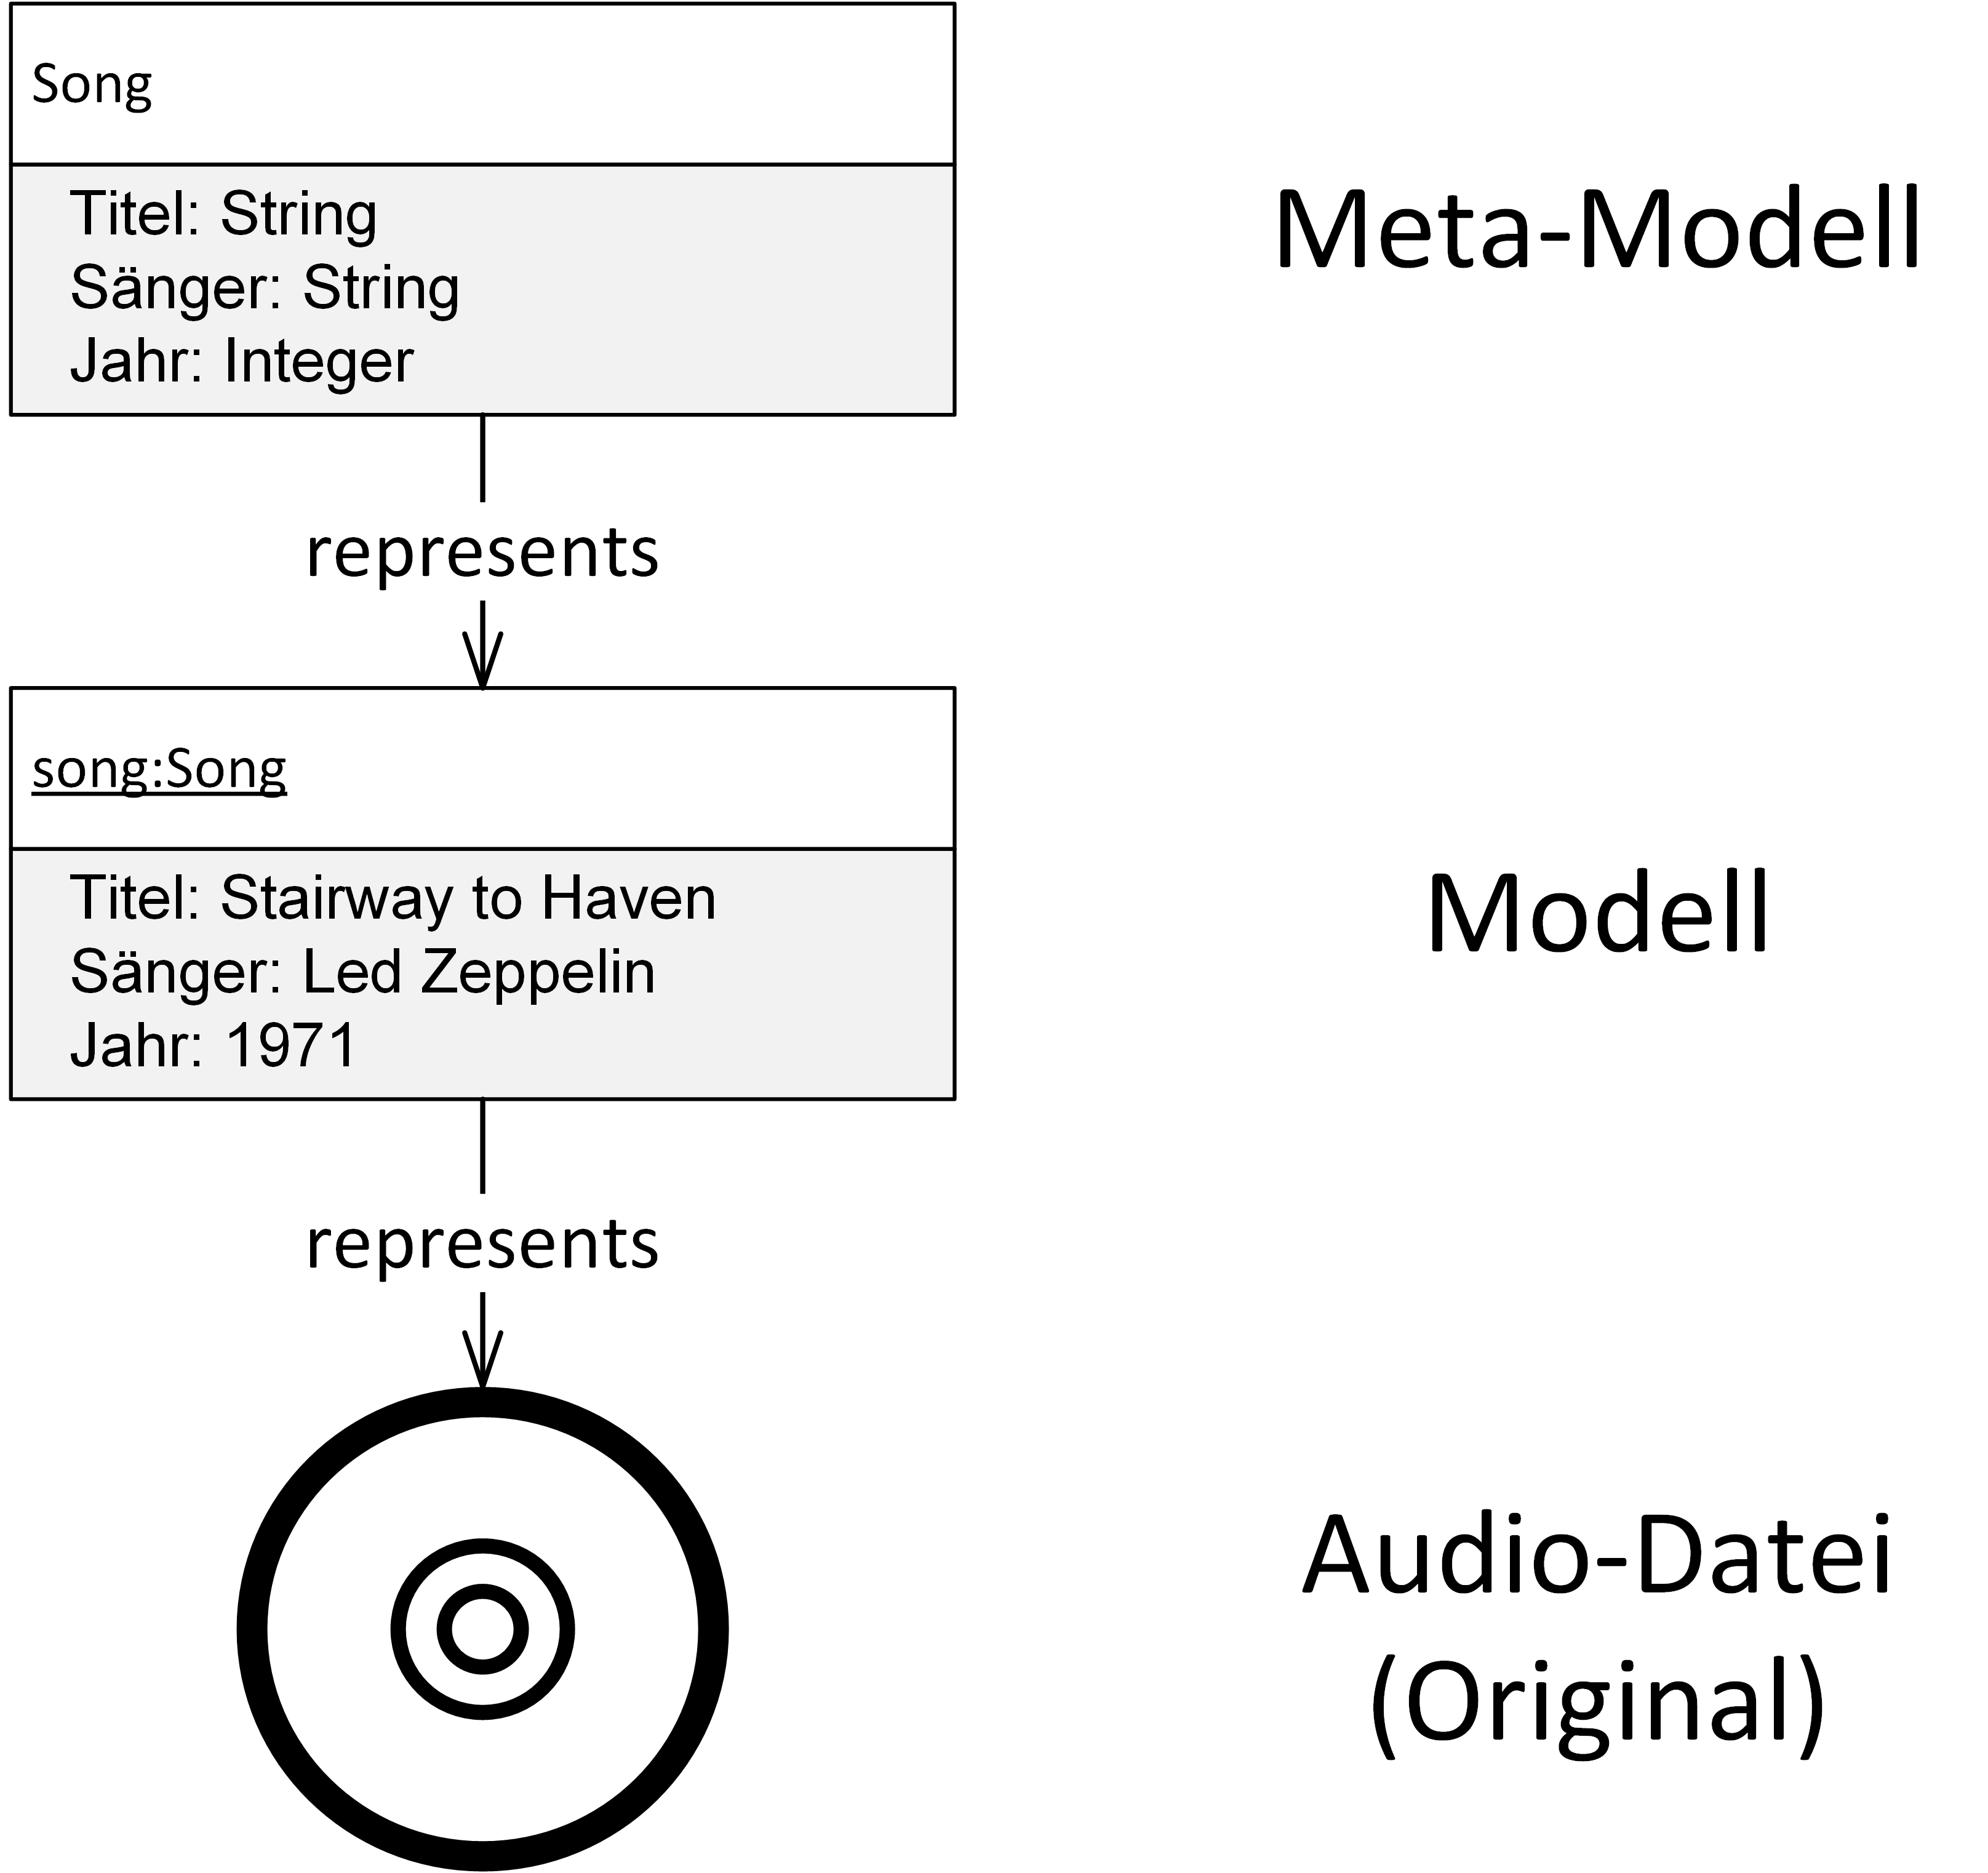
\includegraphics[width=0.55\textwidth]{images/modell_bsp.png}
	\caption{Beziehung zwischen Original, Modell und Meta-Modell}
	\label{img:modell:bsp}
\end{figure}

\subsection{Meta-Modell}
\label{sec:metamodell}
Ein Meta-Modell beschreibt die Struktur eines Modells. In dem Musik-Beispiel aus \autoref{img:modell:bsp}, enthält das Meta-Modell eine Klasse \textbf{Song} mit den Attributen \textbf{Titel}, \textbf{Sänger}, vom Typ String und \textbf{Jahr} vom Typ Integer.
Ein Meta-Modell muss folgende Bereiche abdecken:
\begin{itemize}
\item \textbf{Abstrakte Syntax}: Sie beschreibt die Konstrukte, aus denen die Modelle bestehen, sowie deren Eigenschaften und Beziehungen.
\item \textbf{Konkrete Syntax}: Diese beschreibt die Darstellung der Konstrukte, Eigenschaften und Beziehungen, die in der abstrakten Syntax spezifiziert sind.
\item \textbf{Statische Semantik}: Mithilfe dieser werden Modellierungsregeln und Einschränkungen ausgedrückt, die mit der abstrakten Syntax nicht möglich sind.
\item \textbf{Dynamische Semantik}: Sie drückt die Bedeutung der Konstrukte aus und wird oft nicht formal, sondern durch natürlich sprachlichen Text spezifiziert.
\end{itemize}

\section{Rollen der komponentenbasierten Software-Entwicklung}
\label{sec:rollenSE}
In der komponentenbasierten Softwareentwicklung werden Software-Architektur"=Modelle verwendet. Dabei gibt es vier verschiedene Rollen \cite{Koziolek2006}, die an unterschiedlichen Teilen der Architektur arbeiten und dort ihr spezifisches Wissen einbringen.
\begin{itemize}

\item \textbf{Systemarchitekt}: Die Architektur und der Zusammenhang der einzelnen Komponenten miteinander werden vom Systemarchitekten entworfen. Er ist auch dafür zuständig, weitere Anweisungen an die anderen Rollen weiterzugeben.
\item \textbf{Domänenxperte}: Das Wissen darüber, wie der Benutzer mit dem System interagiert und welche Parameter im Kontrollfluss verwendet werden, stammt vom Domänenxperten.
\item \textbf{Komponentenentwickler}: Für das Implementieren und Spezifizieren der einzelnen Komponenten, ist der Komponentenentwickler verantwortlich.
\item \textbf{Software-Verteilungsexperte}: Die Zusammenstellung der Systemumgebung der Software wird vom Softwareverteilungsexperten übernommen. Außerdem weist der Software-Verteilungsexperte den Ressourcen Komponenten zu.

\end{itemize}


\section{Palladio-Komponentenmodell}
\label{ch:pcm}
Das \gls{pcm} \cite{Becker2010} ist eine Architecture-Description-Language (ADL). Sie wird verwendet, um komponentenbasierte Software zu beschreiben. Neben der Beschreibung sind auch Qualitätsanalysen, wie bezüglich der Performanz oder Zuverlässigkeit möglich. Im Folgenden werden Teile des \gls{pcm} erklärt, die für die Bachelorarbeit wichtig sind.

\subsection{Verwendete Teilmodelle}
\label{sec:submodell}
Das \gls{pcm} unterscheidet ebenfalls in vier verschiedene Rollen. Diese entsprechen den Rollen aus \autoref{sec:rollenSE}. Der einzige Unterschied ist dabei, dass im \gls{pcm} der Systemarchitekt Software-Architekt heißt. Die Aufgaben sind jedoch dieselben. Jede dieser Rollen ist außerdem für ein bestimmtes Submodell zuständig. Die Summe aller Teilmodelle ergibt dann die vollständige Architekturbeschreibung. In \autoref{img:pcm:rollen} sind die Beziehungen zwischen den Rollen und den Submodellen dargestellt. \par
Für das \textbf{Komponenten-Repository-Modell} (Component-Repository-Model) ist der Komponentenentwickler zuständig. Dieses Modell enthält die einzelnen Komponenten und Schnittstellen. Der Software-Architekt ist für das \textbf{Systemmodell} (System-Model) zuständig, das die Zusammensetzung der Komponenten charakterisiert. Der Softwareverteilungsexperte ist für gleich zwei Modelle verantwortlich. Das erste Modell ist das \textbf{Ausführungs-Umgebungs-Modell} (Execution-Environmet-Model). Es beschreibt die benutzte Hardware und das Netzwerk. Das zweite Modell beschreibt wie die einzelnen Komponenten auf der Hardware verteilt werden. Dieses Modell ist das \textbf{Komponenten-Allokations-Modell} (Component-Allocation-Model). Schließlich ist der Domänenxperte für das \textbf{Nutzungsmodell} (Usage-Model) zuständig. Dieses beschreibt die Interaktion des Benutzers mit dem System. \par
Diese Modelle werden im Rahmen der Bachelorarbeit entsprechend um die Möglichkeit zur Modellierung von Datenflüsse und ggf. weiteren für die Vertraulichkeitsanalyse notwendigen Eigenschaften erweitert.
\begin{figure}[h]
	\centering
  	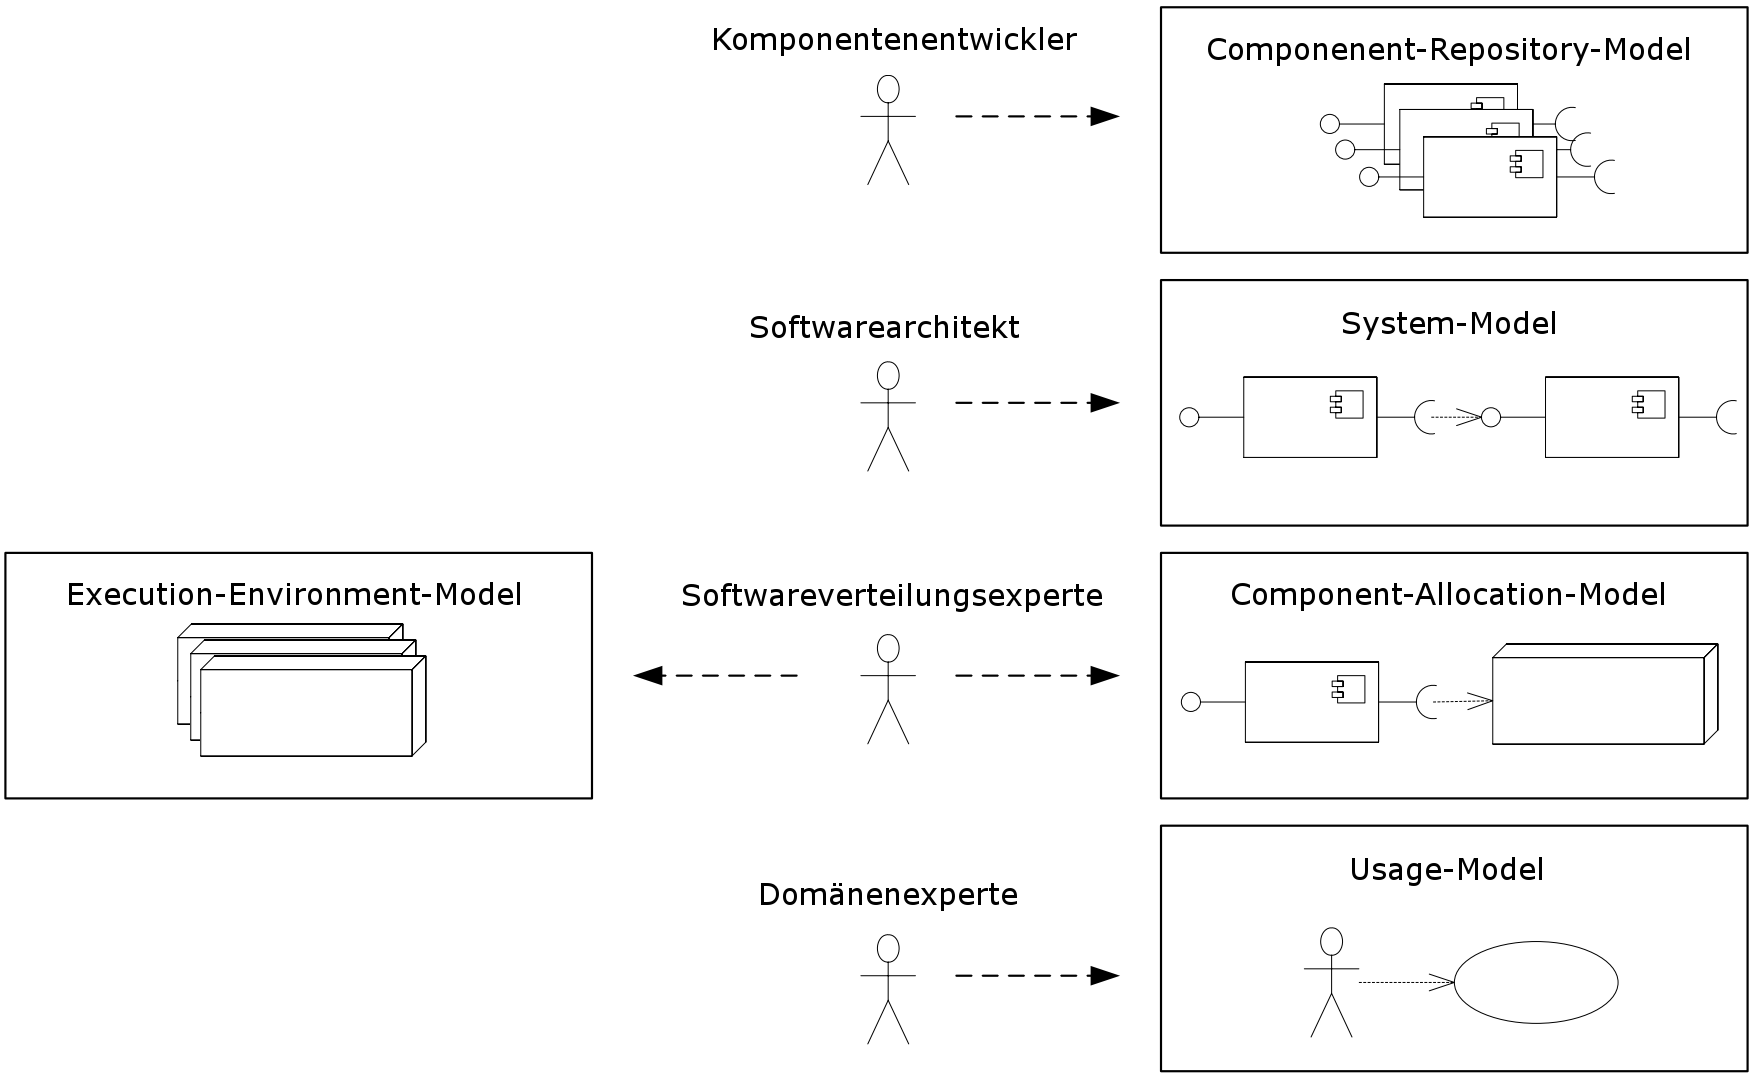
\includegraphics[width=0.9\textwidth]{images/pcm_rollen.png}
	\caption{Beziehung zwischen den Rollen und den Submodellen des PCM}
	\label{img:pcm:rollen}
\end{figure}

\subsection{Service-Effect-Specification}
\label{sec:seff}
Mithilfe der \gls{seff} \cite{Reussner}, kann das Verhalten innerhalb der Komponenten, auf abstrakten und für bestimmte Qualitätsattribute zugeschnittenen Spezfizierungs"=/Detailgrade, beschrieben werden. 
Durch das Spezifizieren von \gls{seff}s kann die Software auf Architekturebene analysiert werden. Dabei gibt es drei verschiedene Abstraktionslevel, die aufeinander aufbauen:
\begin{itemize}
\item \textbf{Signature-List-Based-Interface}: Schnittstellen dienen zur Kommunikation zwischen den Komponenten. Auf dem Signature-List-Based-Interface bauen die anderen Abstraktionslevel auf. Es besteht aus Parametern und Rückgabewerten.
\item \textbf{Protocol-Modeling-Interface}: Mithilfe dieser Schnittstelle lassen sich Aufrufsequenzen definieren.
\item \textbf{Quality-Of-Service-Modelling Interface}: Hier können verschiedene Qualitätsattribute definiert werden.
\end{itemize}
Für Qualitätsanalysen, kann der \gls{seff} in einen endlichen Automaten transformiert werden. Dabei wird ein Aufruf zu einer Komponente als Zustandsübergang modelliert. In \autoref{img:seff:bsp} ist ein \gls{seff} als endlicher Automat dargestellt. Das Beispiel stammt aus \cite{Reussner}. Der \gls{seff} modelliert dabei den Aufruf \texttt{TagWatermarking.download}. Innerhalb des Aufrufs wird \texttt{IDownload.download}, in einer anderen Komponente aufgerufen.
\begin{figure}[h]
	\centering
  	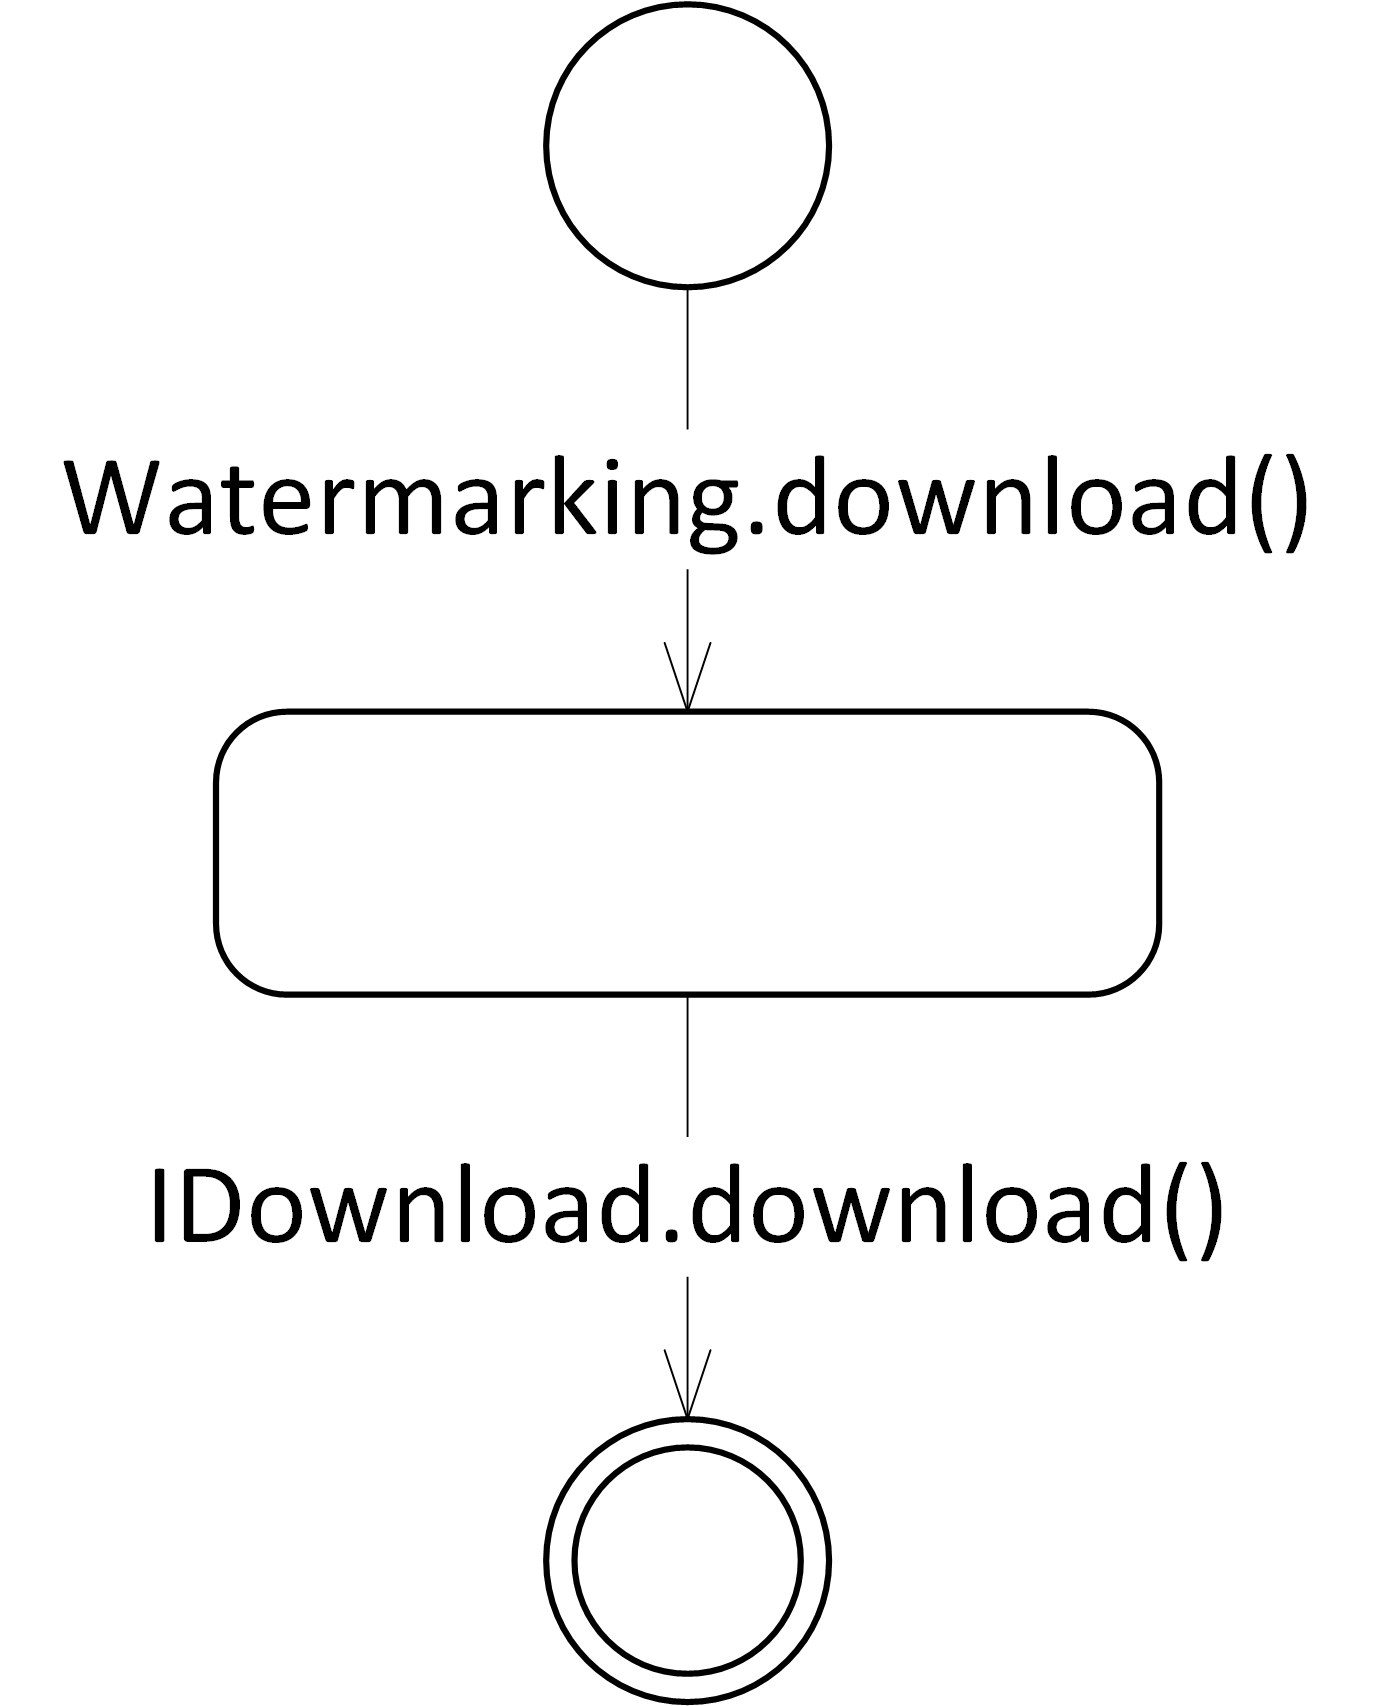
\includegraphics[width=0.3\textwidth]{images/seff_bsp.png}
	\caption{Beispiel SEFF als endlicher Automat}
	\label{img:seff:bsp}
\end{figure} \par
Der \gls{rdseff} ist eine Erweiterung zum \gls{seff}. Die Performanzvorhersage für Komponenten basiert in Palladio, unter anderem, auf der Notation des \gls{rdseff}. In \autoref{img:rdseff:bsp} ist eine Modellierung eines \gls{rdseff} abgebildet. Dabei wurde der Aufruf \texttt{Download} einer \texttt{MediaManagement}-Komponente aus dem Palladio Media-Store modelliert. Das Beispiel stammt aus \cite{Reussner}. Die graphische Darstellung ähnelt dabei der eines UML-Aktivitätsdiagramms, hat aber mit den UML"=Elementen nichts gemeinsam. Der Kontrollfluss beginnt mit dem Ausführen der \texttt{InternalAction} \textbf{JNDI RMI Overhead}. Eine \texttt{InternalAction} repräsentiert dabei einen Aufruf zu Code, der sich innerhalb der Komponente befindet. Außerdem können damit Ressourcen angefordert werden. Im Beispiel werden CPU-Einheiten angefordert. Im Anschluss wird ein \texttt{ExternalCall} ausgeführt, der \textbf{Download} in einer anderen Komponente aufruft, um angeforderte Audio-Dateien zu erhalten. Ein \texttt{ExternalCall} ruft eine Funktion in einer anderen Komponente auf. Schließlich ruft ein weiterer \texttt{ExternalCall} Zip auf, wenn mehr als eine Datei angefordert wurde. Danach endet der Kontrollfluss.
\begin{figure}[h]
	\centering
  	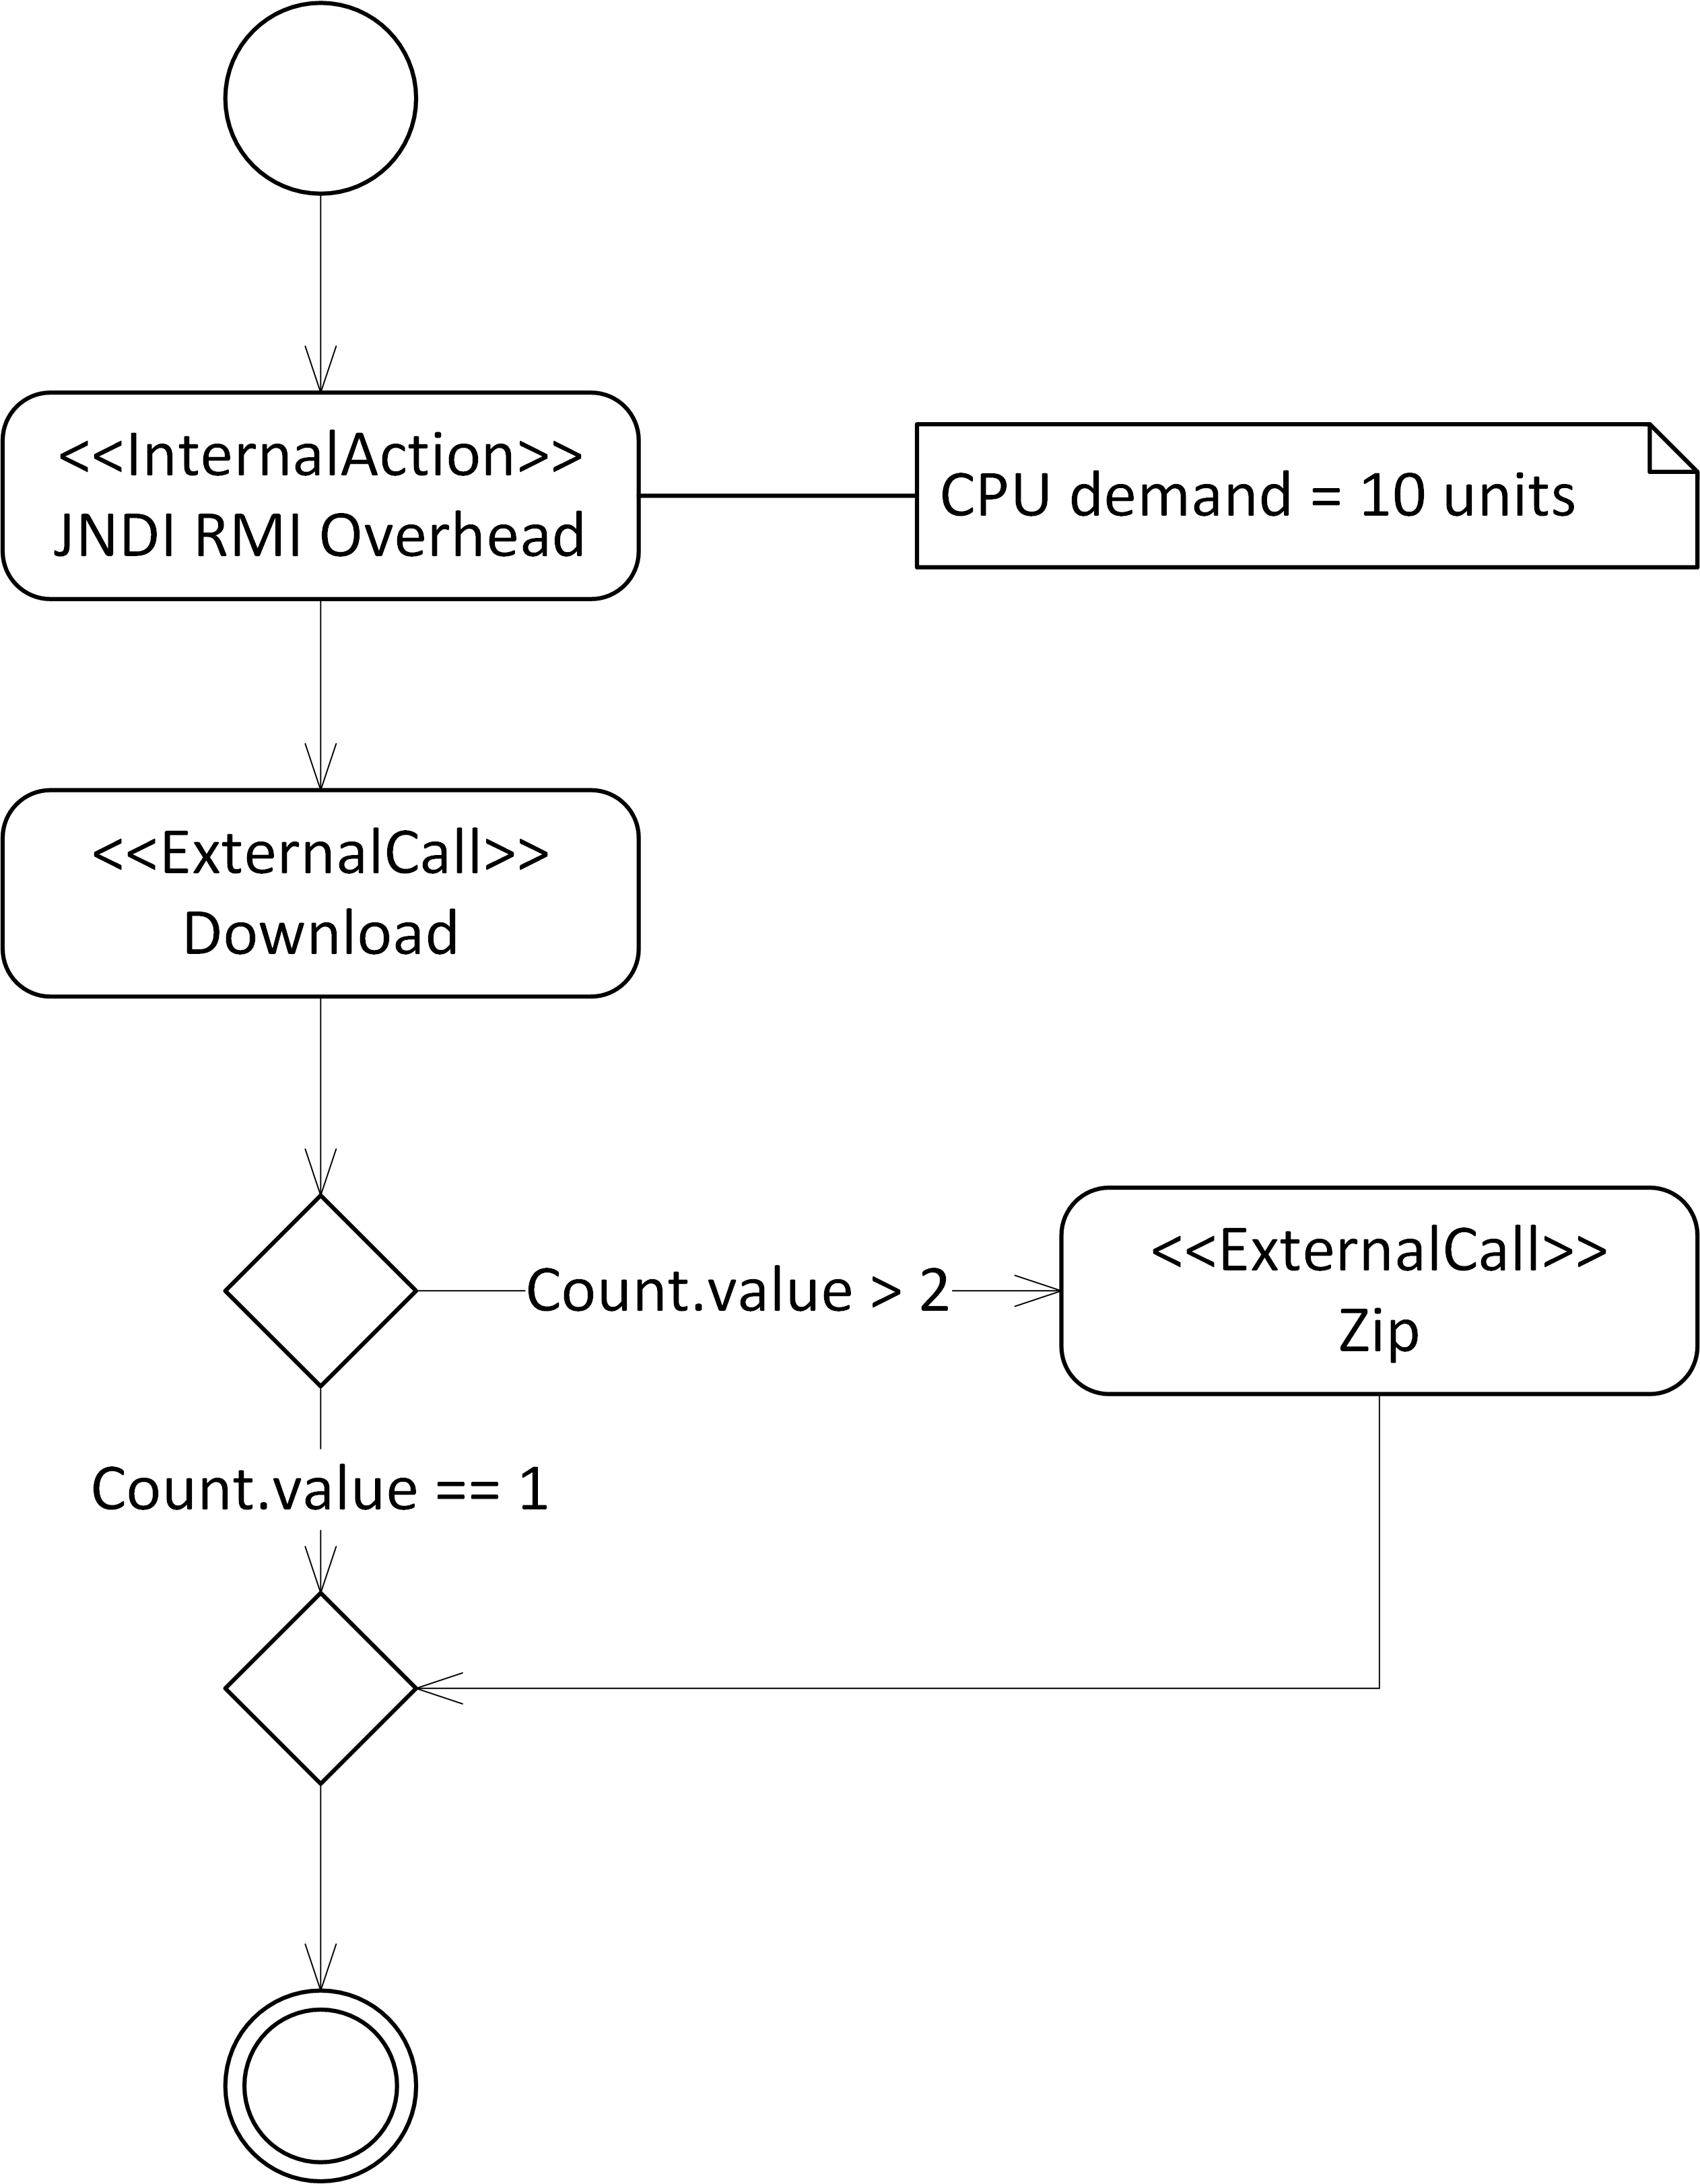
\includegraphics[width=0.6\textwidth]{images/rdseff_bsp.png}
	\caption{RDSEFF, der den Download von Audio-Dateien aus dem Palladio Media-Store modelliert}
	\label{img:rdseff:bsp}
\end{figure} \par
Im Rahmen der Bachelorarbeit soll eine weitere \gls{seff}-Spezialisierung entstehen, die den Datenfluss innerhalb der Komponenten beschreibt.
